\documentclass{article}

\usepackage{amsmath}
\usepackage{amsfonts}
\usepackage{amssymb}
\usepackage{amscd}
\usepackage{amsthm}
\usepackage{graphics}
\usepackage{graphicx}
\usepackage{tikz}

\graphicspath{ {./} }

\title{Auxetic printing software}
\author{Mingruifu Lin, Daniel Wei}
\date{September 2024}

\begin{document}

\maketitle

\begin{abstract}
  Nowadays, too many systems work mechanically, which is very unlike the way the body works. In order to allow larger variety of movements into prosthetics, we have developed smooth structures based on auxetic surfaces. The purpose of this research is to create a software that produces the desired mobile 3D shape from a simple foldable 2D printing. This paper presents the general solution to any such problem.
\end{abstract}

\section{Overview}

\subsection{Mathematical constraints}
The carcass is a 2D differentiable parametric equation $ C: \mathbb{R}^2 \rightarrow \mathbb{R}^3 $. The manifold partition is inherited from the domain partition through $C$. Henceforth, each subset of the partition will be called a "partition-block" in this article.

\subsection{Material constraints}
The production of a tangible object is through 3D printing with either PLA (rigid) or TPU (flexible) plastic entirely. Precision is moderate in general, so attention must be paid to printability when modeling (ex: sufficient gaps, sufficient largeness, etc.)

PLA cannot be bent. It can be brittle. Thus, precision is increased when printing due to its upright rigidity.

TPU can be bent elastically. It is also slightly malleable even cooled state. Thus, precision is lost when printing due to its partial collapse under gravity.

\subsection{Technical constraints}
We chose an auxetic-rubbery model, in which the design structure can exhibits both positive and negative poisson ratio at various points on the manifold. Only tangential forces are allowed, and they can be applied on any partition-block. Tangential forces can also be transmitted from one partition-block to another.

A material is either in "passive mode" or "active mode". Passive mode is achieved when a flat auxetic surface is fully folded into its 3-dimensional structure with no additional force apart from its intrinsic forces. However, there can still be degrees of freedom baked into the structure: active mode is achieved when one or more degrees of freedom are used to further change the shape of the manifold. Active mode allows our auxetic surface to change shape when acted upon by a motor, for example.

When the usage of the auxetic surface involves fluid transport or storage, the structure can be covered with a thin, elastic-enough material, in order to preserve the structure's active mode. More blunt forces do not require auxetic technology: a simple mechanical system is sufficient; auxetic technology is used for milder body motion.


\section{Theoretical aspects}

\subsection{Mathematical model}
Recall that our auxetic surface is modelled by a parametric function $ C: A \rightarrow \mathbb{R}^3 $, where $A \subset \mathbb{R}^2$ is a bounded, connected subset with the standard topology; for the sake of identifying variables, we write $ C: (s, t) \rightarrow (x, y, z) $. When the flat surface is folded into its 3-dimensional shape, two events occur at each point:
1. The surface expands or retracts at that point.
2. The surface curves at that point.

\subsubsection{Expansion}
The expansion at each point is the 2-tuple of its expansions along $s$ and $t$, which can be computed with the magnitudes of the derivatives with respect to $s$ and $t$. If radial symmetry is present, we can simply consider the divergence of the derivative (which is a vector field) at the point.

\subsubsection{Curvature}
A consistent oriented curvature for a manifold can be computed by multiplying the point's curvature with the magnitude of the normal/cross-product of the tangent vectors in the order $s, t$. The tangent vectors can be computed, again, using the derivatives with respect to $s$ and $t$. The order of the cross-product must be kept throughout the algorithm, in order to preserve a well-defined orientation. This normal vector is then multipled by the unsigned curvature.

\subsubsection{Tiling}
Recall that we are also partitioning the manifold, so we consider many possible tesselations. Tiling significantly influences the auxetic shape used. Each tile's center can represent a partition-block and the edges can be arbitrary links shared between the connected partition-blocks. As well, we can consider the dual tesselation: each vertex is a partition-block and each edge is a link.

There only exists 3 regular tilings: triangular, square, hexagonal. Regular tilings are preferable to general monohedral tilings due to ... their regularity; they are easier to work with. However, let us not discount the fact that general monohedral tilings could arise as optimal tilings in some unique situations.

There only exists 8 semi-regular tilings; they use one or more regular polygons to tile. The interest arises when assigning roles to each polygon (some can serve as "faces" whilst others can serve as mobile links).

As well, many non-edge-to-edge tilings benefit from this role assignation.

Other tilings involving multiple non-regular shapes, that are either edge-to-edge or non-edge-to-edge are possible, and are definitely worth exploring later.

For the sake of quickly crafting a working project, we are restricting ourselves to regular square tilings. A single square has a total of 4 links, one for each adjacent square. Its dual tesselation also happens to be itself. Also, any visibly non-random, non-edge-to-edge square tiling is clearly isomorphic to an edge-to-edge square tiling in the dual tesselation space (by rotating one's perspective about the z-axis).

Evidently, there is much more to tiling, such as the wallpaper group or Voronoi tilings.

\subsection{Auxetic behaviors}
Instead of considering the manifold as a set of points, the manifold is partitioned into partition-blocks to allow implementation of auxetics. Thus, each partition-block undergoes a combo of approximated expansion and curvature. For each combo, there exists a continuum of auxetic shapes that do the job. TPU's flexibility gives the necessary leeway for the approximations' applicability.

\subsubsection{Radial auxetics}

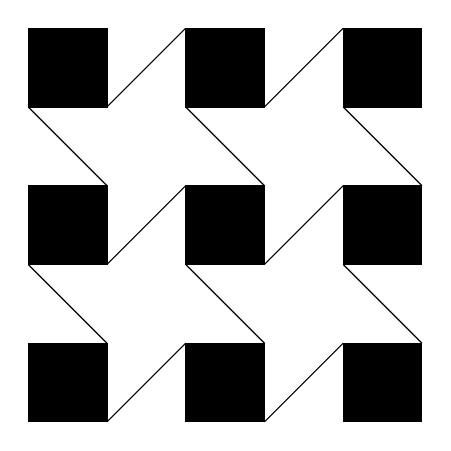
\begin{tikzpicture}
  \filldraw[color = black!100] (0, 0) rectangle (1, 1);
  \filldraw[color = black!100] (2, 0) rectangle (3, 1);
  \filldraw[color = black!100] (4, 0) rectangle (5, 1);

  \filldraw[color = black!100] (0, 2) rectangle (1, 3);
  \filldraw[color = black!100] (2, 2) rectangle (3, 3);
  \filldraw[color = black!100] (4, 2) rectangle (5, 3);

  \filldraw[color = black!100] (0, 4) rectangle (1, 5);
  \filldraw[color = black!100] (2, 4) rectangle (3, 5);
  \filldraw[color = black!100] (4, 4) rectangle (5, 5);

  \draw (1, 0) -- (2, 1);
  \draw (1, 2) -- (2, 3);
  \draw (1, 4) -- (2, 5);
  \draw (3, 0) -- (4, 1);
  \draw (3, 2) -- (4, 3);
  \draw (3, 4) -- (4, 5);

  \draw (1, 1) -- (0, 2);
  \draw (3, 1) -- (2, 2);
  \draw (5, 1) -- (4, 2);
  \draw (1, 3) -- (0, 4);
  \draw (3, 3) -- (2, 4);
  \draw (5, 3) -- (4, 4);
\end{tikzpicture}

\vspace{5mm}

Consider the central square. By rotating, it expands in all directions. If we rotate them back, they contract to their original state.

This is the defining feature of negative poisson ratio: the magnitudes of the orthogonal derivatives at each point are either both positive or both negative.

Expansion is determined by the ratio between the block size and the gap size. A higher block size to gap size produces a bigger expansion.

We have considered more extreme rotational auxetics such as the following:

\includegraphics[width = 10cm]{extreme-auxetic.jpeg}

\vspace{5mm}

The expansion range is almost doubled if the blocks fully rotate. However, due to flexibility constraint, we will stick with the diagonals.

\subsubsection{Longitudinal auxetics}
Structures with positive poisson ratio will be referred as longitudinal auxetics. (They are not auxetics properly speaking, but the goal is to unify the terms employed.)

The defining feature of positive poisson ratio is the inverted relationship between the magnitudes of the orthogonal derivatives at each point: one is positive, the other is negative. In other words, the expansion in a direction led to the retraction in the other direction.

\vspace{5mm}

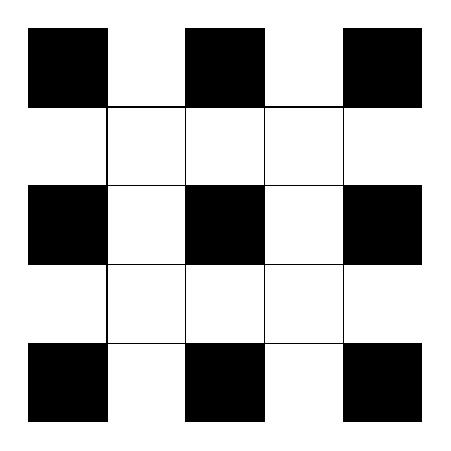
\begin{tikzpicture}
  \filldraw[color = black!100] (0, 0) rectangle (1, 1);
  \filldraw[color = black!100] (2, 0) rectangle (3, 1);
  \filldraw[color = black!100] (4, 0) rectangle (5, 1);

  \filldraw[color = black!100] (0, 2) rectangle (1, 3);
  \filldraw[color = black!100] (2, 2) rectangle (3, 3);
  \filldraw[color = black!100] (4, 2) rectangle (5, 3);

  \filldraw[color = black!100] (0, 4) rectangle (1, 5);
  \filldraw[color = black!100] (2, 4) rectangle (3, 5);
  \filldraw[color = black!100] (4, 4) rectangle (5, 5);

  \draw (1, 2) -- (2, 2);
  \draw (1, 4) -- (2, 4);
  \draw (3, 2) -- (4, 2);
  \draw (3, 4) -- (4, 4);

  \draw (1, 1) -- (2, 1);
  \draw (1, 3) -- (2, 3);
  \draw (3, 1) -- (4, 1);
  \draw (3, 3) -- (4, 3);

  \draw (1, 1) -- (1, 2);
  \draw (3, 1) -- (3, 2);
  \draw (1, 3) -- (1, 4);
  \draw (3, 3) -- (3, 4);

  \draw (2, 1) -- (2, 2);
  \draw (4, 1) -- (4, 2);
  \draw (2, 3) -- (2, 4);
  \draw (4, 3) -- (4, 4);
\end{tikzpicture}

\vspace{5mm}

In the diagram, pulling in one diagonal direction retracts the structure in the other diagonal direction.

\subsubsection{Free auxetics}
Some structures allow free stretching in one direction, but do not expand nor retract in the other direction. This corresponds to a null poisson ratio. Again, this word is invented, and does not exist, but will be used in this paper.

\subsubsection{Non-auxetics}
Non-auxetics do not expand or retract in the transverse direction when pulled or compressed. The simplest example is the juxtaposition between a block and its adjacent ones. (Each block itself is non-auxetic!) The poisson ratio is undefined in this case.

\subsubsection{Perpendicular protrusion}
To achieve a desired "consistent signed curvature", a structure must protrude either exclusively inwards or exclusively outwards when subjected to expansion/retraction, depending on the manifold orientation set by the engineer. In other words, we eliminate bistable cases.

Simple example is the following:

\vspace{5mm}

\includegraphics[width = 10cm]{perp-protrusion.jpeg}

\vspace{5mm}

This is a side-view for two partition-blocks. When stretched, the left one naturally becomes lower than the right one. This rod can be set diagonally to also allow expansion.

\subsection{Composing in $\mathbb{R}^2$}

\subsubsection{Discrete remapping}
Now, we enter the crux of the idea: we want the 2D surface to fold into its 3D shape.

Our method is to remap the points in $A \subset \mathbb{R}^2$:

1. Compute the divergence (scalar field) of the derivatives of the parametric surface.
2. Partition $A$ into squares, and keep only and all the vertices.
3. Move adjacent points nearer or farther depending on the divergence at each point. A high divergence needs more points to fill the gap, so points move closer to high divergence points.

Notice we are only keeping the points. Now each point is a partition-block, and can be customized depending on the desired auxetic property. We want to choose an auxetic shape for each point such that all remapped points go back to their original position; thus, when we stretch the printed surface, all partition-blocks will start to evenly spread out in 3D. Divergence is acting as substitute for distance (since the mathematics deal with continuous shapes).

\subsubsection{Even reparametrization}
There is an infinite number of parametrization for a given surface. A good paramatrization should ideally have very evenly spaced gridlines, i.e. the magnitude of the derivatives with respect to $s$ and $t$ should be relatively constant. This is because we want to keep the 2D printed auxetic surface's high resolution when it is expanded/folded into its passive 3D version. If the divergence is too high at a point, it will be very crowded on the 2D printed surface. We haven't found a way yet, but we should always try to choose a good parametrization when using this algorithm.

\end{document}
